\section{Руководство пользователя}
\label{sec:user_guide}

\subsection{Старт сервера} 
\label{sec:user_guide:serverstart}

Для того, чтобы запустить сервер, необходимо воспользоваться запуском приложения с параметрами командной строки. Сделать это можно двумя способами: используя командную строку и используя ярлык с параметрами. Рассмотрим каждый из способов. 
Для того, чтобы запустить сервер с помощью командной строки, необходимо открыть командную строку, перейти в папку с исполняемым файлом, выполнить программу со следующими аргументами: адрес сервера, порт сервера, максимальное количество активных соединений (Рисунок \ref*{sec:user_guide:serverstart:conrunargs}). В результате появится консольное окно сервера c сообщением об успешном запуске и текущем адресе сервера (Рисунок \ref*{sec:user_guide:serverstart:runres}). 
Для того, чтобы использовать второй подход, необходимо создать ярлык приложения, и после пути добавить аргументы через пробел (Рисунок \ref*{sec:user_guide:serverstart:shortcut}). Как и в предыдущем случае, индикатором успешного запуска будет является сообщение с текущем адресом сервера (Рисунок \ref*{sec:user_guide:serverstart:runres}).

\begin{figure}[ht]
	\centering
	  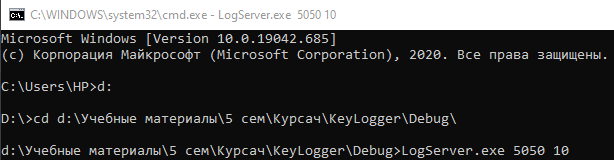
\includegraphics[scale=0.9]{attachments/conrunargs.png}  
	  \caption{ Команда запуска сервера с параметрами }
	  \label{sec:user_guide:serverstart:conrunargs}
\end{figure}

\begin{figure}[ht]
	\centering
	  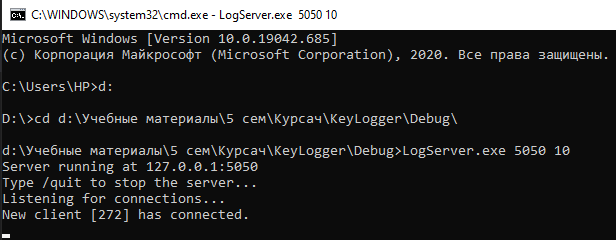
\includegraphics[scale=0.9]{attachments/runres.png}  
	  \caption{ Результат запуска сервера }
	  \label{sec:user_guide:serverstart:runres}
\end{figure}

\begin{figure}[ht]
	\centering
	  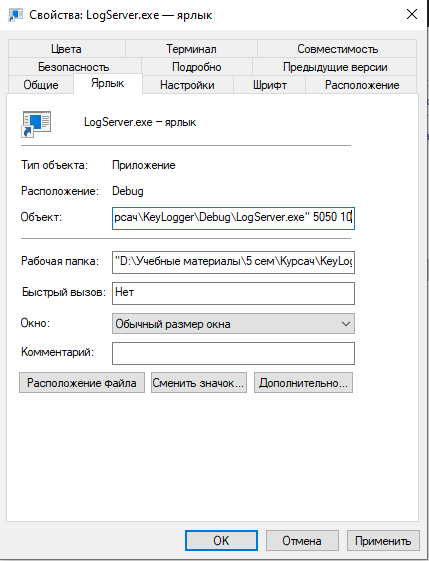
\includegraphics[scale=1]{attachments/shortcut.png}  
	  \caption{ Параметры запуска в ярлыке }
	  \label{sec:user_guide:serverstart:shortcut}
\end{figure}

\subsection{Остановка сервера} 
\label{sec:user_guide:serverstop}

Для того, чтобы остановить сервер, можно воспользоваться командой /quit. Настоятельно рекомендуется завершать сервер именно этой командой, а не закрытием консольного окна, так как в этом случае все логи гарантированно запишутся на диск, чего может не произойти при некорректном закрытии. 

\subsection{Единоразовая настройка программного средства мониторинга пользовательского ввода} 
\label{sec:user_guide:keyloggersetup}

Для того, чтобы программное средство успешно продолжало работать само по себе, необходимо корректно провести начальную настройку. Для этого необходимо запустить исполняемый файл с параметрами командной строки аналогичными способами, описанными в руководстве по запуску сервера. Программа принимает следующие аргументы: адрес сервера, порт сервера, количество символов до отправки на сервер. В случае успешного запуска пользователь не получит никакого сообщения. Проверить, что программа работает можно в диспетчере задач Windows (Рисунок \ref*{sec:user_guide:keyloggersetup:keyloggertask}).

\begin{figure}[ht]
	\centering
	  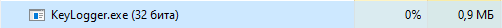
\includegraphics[scale=0.9]{attachments/keyloggertask.png}  
	  \caption{ Программное средство мониторинга пользовательского ввода в диспетчере задач }
	  \label{sec:user_guide:keyloggersetup:keyloggertask}
\end{figure}
